% Signal Scissors comprehensive study guide.
% Compile from this directory with pdfLaTeX (twice): pdflatex signal_scissors_study_guide.tex
\documentclass[11pt,a4paper]{article}
\usepackage[margin=24mm,headheight=14pt]{geometry}
% pdfLaTeX font setup.  Prism/Overleaf installs normally provide both packages.
% The fallbacks keep the document compilable in smaller TeX installations.
\usepackage[T1]{fontenc}
\usepackage[utf8]{inputenc}
\IfFileExists{lato.sty}{\usepackage[default]{lato}}{\usepackage{lmodern}}
\IfFileExists{montserrat.sty}{\usepackage[defaultfam]{montserrat}}{\usepackage{helvet}}
\usepackage{microtype,graphicx,booktabs,array,tabularx,longtable,amsmath,amssymb,mathtools}
\usepackage[dvipsnames]{xcolor}
\usepackage{enumitem,csquotes,fancyhdr,hyperref,tcolorbox,caption,float,siunitx,titlesec}
\usepackage{tikz}
\usetikzlibrary{arrows.meta,positioning,shapes.geometric}
\hypersetup{colorlinks=true,linkcolor=MidnightBlue,urlcolor=MidnightBlue,citecolor=MidnightBlue,pdftitle={Signal Scissors Study Guide}}
\definecolor{ink}{HTML}{172033}
\definecolor{blue}{HTML}{2563EB}
\definecolor{teal}{HTML}{0F766E}
\definecolor{soft}{HTML}{EFF6FF}
\definecolor{warn}{HTML}{92400E}
\titleformat{\section}{\sffamily\Large\bfseries\color{ink}}{\thesection}{0.75em}{}
\titleformat{\subsection}{\sffamily\large\bfseries\color{ink}}{\thesubsection}{0.65em}{}
\titleformat{\subsubsection}{\sffamily\normalsize\bfseries\color{ink}}{\thesubsubsection}{0.55em}{}
\titlespacing*{\section}{0pt}{2.4ex plus .7ex minus .2ex}{1.15ex}
\titlespacing*{\subsection}{0pt}{1.85ex plus .5ex minus .2ex}{.85ex}
\titlespacing*{\subsubsection}{0pt}{1.45ex plus .4ex minus .15ex}{.65ex}
\linespread{1.08}\selectfont
\setlength{\parskip}{0.78em}
\setlength{\parindent}{0pt}
\renewcommand{\arraystretch}{1.22}
\setlength{\intextsep}{1.25em plus .25em minus .2em}
\setlist[itemize]{leftmargin=1.5em,itemsep=0.25em}
\setlist[enumerate]{leftmargin=1.7em,itemsep=0.3em}
\pagestyle{fancy}\fancyhf{}\lhead{\sffamily\small Signal Scissors}\rhead{\sffamily\small Study Guide}\cfoot{\thepage}
\newcommand{\code}[1]{\texttt{#1}}
\newcommand{\fig}[2]{\begin{figure}[H]\centering\includegraphics[width=\linewidth]{figures/#1}\caption{#2}\end{figure}}
\newtcolorbox{intuitive}{colback=soft,colframe=blue!60!black,title=Start with the idea,fonttitle=\sffamily\bfseries,breakable}
\newtcolorbox{implementation}{colback=teal!5,colframe=teal!70!black,title=What this project actually does,fonttitle=\sffamily\bfseries,breakable}
\newtcolorbox{viva}{colback=yellow!8,colframe=warn,title=Viva checkpoint,fonttitle=\sffamily\bfseries,breakable}
\newtcolorbox{formula}{colback=white,colframe=black!35,boxrule=.35pt,arc=1mm,left=4mm,right=4mm,top=2.5mm,bottom=2.5mm,boxsep=0pt}
\newcommand{\applied}[3]{\begin{tcolorbox}[colback=white,colframe=black!28,boxrule=.3pt,arc=1mm,left=3mm,right=3mm,top=1.8mm,bottom=1.8mm]\small\textbf{Where applied:} #1\par\textbf{Why it matters:} #2\par\textbf{How it is applied:} #3\end{tcolorbox}}
% Put all \[ ... \] display equations in a thin, neutral formula box.
\let\SSDisplayMath\displaymath
\let\endSSDisplayMath\enddisplaymath
\renewenvironment{displaymath}{\begin{formula}\SSDisplayMath}{\endSSDisplayMath\end{formula}}
\newcommand{\term}[1]{\textbf{#1}}

\begin{document}
\begin{titlepage}
\centering
\vspace*{2.5cm}
{\sffamily\fontsize{30}{36}\selectfont\bfseries Signal Scissors\par}
\vspace{0.35cm}
{\sffamily\Large Comprehensive Study, Demonstration, and Viva Guide\par}
\vspace{1.2cm}
\begin{tcolorbox}[width=.88\textwidth,colback=soft,colframe=blue!65!black]
An implementation-grounded guide to the Signal Scissors audio DSP workstation. It explains the user interface, the signal path, the mathematics, actual algorithms, demonstrations, and likely viva questions.
\end{tcolorbox}
\vfill
{\large CSE 220 --- Signals \& Systems Sessional\par}
{\large Department of CSE, BUET\par}
\vspace{0.6cm}
{\small Figures in this guide are generated deterministically by \code{generate\_figures.py}; they use the same equations and parameter choices as the backend examples.\par}
\end{titlepage}

\tableofcontents
\newpage

\section{Project overview}
Signal Scissors is an interactive digital signal-processing (DSP) workstation for audio. A person can load a file, record from a microphone, or create known test signals; examine the waveform and spectrum; process the signal; listen to it; compare it with the original; and export the result. The central learning goal is to connect an audible change to a visible and mathematical change.

The active application is a React/Vite frontend and a Python FastAPI backend. NumPy and SciPy perform the core numerical work. The current session is held in backend memory: it is a lab workstation rather than a multi-user audio archive.

\begin{intuitive}
Audio is a sequence of measured air-pressure values. In the \emph{time domain} we ask ``how did the amplitude move over time?'' In the \emph{frequency domain} we ask ``which repeating speeds (frequencies) are present, and how strong are they?'' Signal Scissors lets the user move between these two useful views.
\end{intuitive}

\subsection{What the user can do}
\begin{itemize}
\item Load WAV directly, or use FFmpeg decoding for other supported browser-uploaded audio formats when FFmpeg is installed; record a microphone signal; or load four teaching presets.
\item Apply an FFT band operation: \emph{cut}, \emph{keep}, \emph{attenuate}, or \emph{amplify} a selected frequency range.
\item Apply gain, a zero-padded delay, analytic single-sideband (SSB) frequency translation, a multi-tap convolution echo, and six voice transformations.
\item Inspect original and processed waveform, magnitude spectrum, STFT spectrogram, RMS, peak, dominant frequency, and an echo impulse response.
\item Use one-click real-life preset chains; denoise the current signal with an STFT spectral gate; A/B play and export processed PCM WAV.
\end{itemize}

\section{System architecture and complete processing flow}
\begin{center}
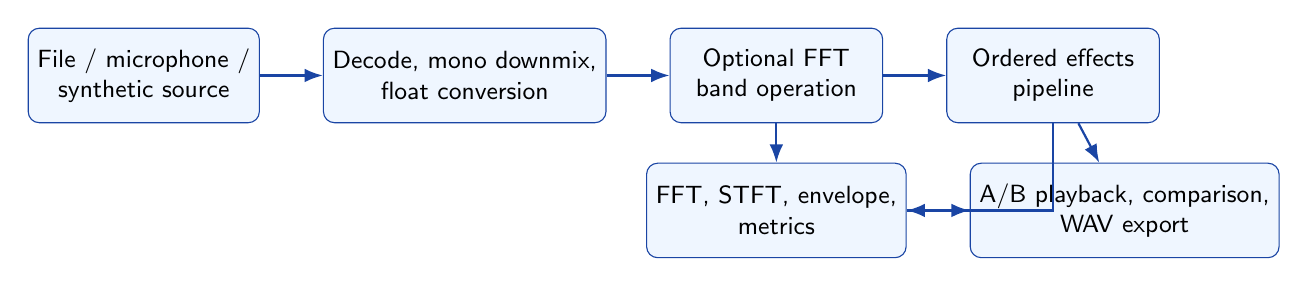
\begin{tikzpicture}[node distance=5mm and 8mm, every node/.style={font=\sffamily\small,align=center}, box/.style={draw=blue!70!black,rounded corners,fill=soft,minimum height=12mm,minimum width=27mm}, arr/.style={-Latex,thick,blue!70!black}]
\node[box] (input) {File / microphone /\\synthetic source};
\node[box,right=of input] (decode) {Decode, mono downmix,\\float conversion};
\node[box,right=of decode] (filter) {Optional FFT\\band operation};
\node[box,right=of filter] (effects) {Ordered effects\\pipeline};
\node[box,below=of filter] (analysis) {FFT, STFT, envelope,\\metrics};
\node[box,right=of analysis] (out) {A/B playback, comparison,\\WAV export};
\draw[arr] (input)--(decode);\draw[arr](decode)--(filter);\draw[arr](filter)--(effects);\draw[arr](effects)--(out);\draw[arr](filter)--(analysis);\draw[arr](effects)|-(analysis);\draw[arr](analysis)--(out);
\end{tikzpicture}
\end{center}

\subsection{Actual route and state behaviour}
The backend has an original signal, an intermediate frequency-filtered signal, and a current processed signal. A filter or effect may target the original track or the current processed track. This makes chained experiments possible, but it also means a presenter should reset before an experiment if a clean before/after comparison is desired. The full pipeline endpoint performs:
\[
\boxed{\text{FFT filter}\ \longrightarrow\ \text{gain}\ \longrightarrow\ \text{delay}\ \longrightarrow\ \text{SSB shift}\ \longrightarrow\ \text{voice effect}\ \longrightarrow\ \text{echo}.}
\]
The app clips only when WAV bytes are created for listening/export; the echo additionally uses a soft \(\tanh\) limiter only if its convolution output exceeds magnitude 1. Intermediate gain is deliberately not hard-clipped.

\subsection{User-guide quick start}
\begin{enumerate}
\item In \emph{Control Center}, load \emph{Standard Multi-Tone}. It contains 200, 1000, and 2500 Hz components plus random Gaussian noise.
\item Open \emph{DSP Studio}; enable Filter; set 900--1100 Hz and choose Cut; apply to Original.
\item In the spectrum, find the 1000 Hz peak before processing and its disappearance afterward. Listen using the original/processed toggle.
\item Open \emph{Signal Inspector} to discuss waveform overlay, spectral difference, STFT, RMS, peak, and dominant frequency.
\item Reset before the next independent experiment. For echo, load \emph{Acoustic Pulse Burst}, not a continuous tone: separated repeats are far easier to see and hear.
\end{enumerate}

\section{Input audio and signal representation}
For a sampling rate \(f_s\) samples/s (Hz), the computer stores samples \(x[n]\), where \(n\) is an integer. Their time is \(t_n=n/f_s\). A sampled sine wave is
\[
x[n]=A\sin\left(2\pi f\frac{n}{f_s}+\phi\right).
\]
The sampling interval is \(T_s=1/f_s\). The highest frequency that can be represented without aliasing is the \term{Nyquist frequency}, \(f_N=f_s/2\). For the supplied 8 kHz synthetic signals, \(f_N=4\) kHz. The API rejects a band upper cutoff above Nyquist.
\applied{Every input route, the sample-rate/Nyquist status display, custom sine generator, and filter cutoff validation.}{It prevents the user from requesting frequencies that the sampled audio cannot represent uniquely.}{The backend records the file's \(f_s\), uses it to label graphs and FFT bins, and checks the filter's upper edge against \(f_s/2\).}

\subsection{Sources and preprocessing}
\begin{longtable}{p{.21\linewidth}p{.36\linewidth}p{.35\linewidth}}
\toprule Source & User action & Actual signal created or accepted \\\midrule
Standard multi-tone & Click preset \code{tones} & 2 s at 8 kHz: 200, 1000, 2500 Hz sines, \(+0.3\) Gaussian noise, then peak-normalised.\\
Harmonic multi-tone & Click \code{multitone} & 150, 440, 1200, 3200 Hz plus Gaussian noise, peak-normalised.\\
Pulse burst & Click \code{pulse} & A 440 Hz, 180 ms Hann-windowed burst beginning at 80 ms; low noise is added. Intended for delay/echo.\\
Tone + white noise & Click \code{noise} & 300 Hz sine plus strong independent Gaussian white noise, then peak-normalised.\\
File upload & Browse or drop a file & WAV is decoded with SciPy; other formats require FFmpeg. Stereo is averaged to mono in \code{load\_wav}. Integer PCM becomes floating point approximately in \([-1,1]\).\\
Microphone & Record, listen back, Use Recording & Browser decodes the captured blob, averages channels to mono, and encodes 16-bit PCM WAV before upload.\\
\bottomrule
\end{longtable}

\subsection{Generator, academy, settings, and playback modules}
The \emph{Signal Generator \& Capture Lab} also creates a custom pure sine in the browser. The user selects \(f_0\) and duration; the browser chooses \(f_s=\max(8000,\min(240000,\lceil2.4f_0\rceil))\), writes \(x[n]=\sin(2\pi f_0n/f_s)\), encodes 16-bit mono WAV, and uploads it. The 2.4 factor gives headroom over twice the target frequency, though Nyquist's ideal condition is strictly greater than \(2f_0\). This is the most controlled input for testing one spectral peak.

DSP Academy is an in-app teaching page: it displays DFT, Nyquist/aliasing, convolution, analytic SSB, denoising, and band-filter explanations plus six interactive canvas simulations. It teaches and visualises; it does not alter the backend's audio signal. The Signal Inspector and Studio canvas use the backend payloads, whereas the Theory simulations are browser-side illustrations.

The transport bar supports original/processed A/B listening, seek, volume, and WAV export. Settings offers light/dark/system appearance and display preference toggles. The backend export endpoint currently always produces clipped 16-bit PCM WAV; the Settings page's ``32-bit Float WAV'' selector is currently a UI selection and does not change that endpoint. Reset returns to original, and the full Settings reset additionally reloads the standard test tone.

\begin{viva} Why does downmixing matter? Averaging stereo channels produces one channel so the current DSP functions receive a one-dimensional signal. It is convenient for teaching, but opposite-polarity left/right content can partially cancel, and stereo spatial information is not preserved.
\end{viva}

\section{Seeing the signal: waveform, spectrum, and spectrogram}
The backend computes a full FFT for processing and a one-sided real FFT for display. For \(N\) samples, the DFT is
\[
X[k]=\sum_{n=0}^{N-1}x[n]e^{-j2\pi kn/N},\qquad
x[n]=\frac{1}{N}\sum_{k=0}^{N-1}X[k]e^{j2\pi kn/N}.
\]
The physical frequency of bin \(k\) is \(f_k=kf_s/N\). The display magnitude is \(|X[k]|/N\); its interior positive-frequency bins are doubled because a real waveform has mirror-image negative-frequency content. DC and, for even \(N\), Nyquist are not doubled.

A \term{spectrogram} repeats a short-time Fourier transform (STFT) on overlapping pieces of audio. It answers ``which frequencies were strong at which time?'' The project uses SciPy's spectrogram with up to a 256-sample window and 50\% overlap for visualisation. Its plotted magnitude is converted to dB using \(20\log_{10}(\max(|S|,10^{-6}))\). The waveform sent to the browser is a min/max envelope (up to 1200 values) so a long waveform remains quick to draw without hiding narrow peaks.
\applied{Studio, Signal Inspector, microphone preview, and Noise Remover comparisons.}{A waveform exposes timing and amplitude, an FFT exposes stationary components, and an STFT reveals how frequency content changes over time.}{The backend sends a downsampled min/max waveform, a one-sided dB FFT, and an STFT grid to the React canvas visualisers.}

\section{Applied theories and concepts}
Table~\ref{tab:applied-theories} is a compact reference for the mathematical ideas used by Signal Scissors. It distinguishes the theoretical name from the practical feature so it can be used for revision or during a viva.

{\small
\setlength{\tabcolsep}{2pt}
\renewcommand{\arraystretch}{1.3}
\begin{longtable}{@{}p{.19\linewidth}p{.26\linewidth}p{.25\linewidth}p{.22\linewidth}@{}}
\caption{Applied theories and concepts in Signal Scissors}\label{tab:applied-theories}\\
\toprule
\textbf{Name of theory / concept} & \textbf{Equations and formulas} & \textbf{Short description} & \textbf{Where applied in the app}\\
\midrule
\endfirsthead
\multicolumn{4}{l}{\small\itshape Table~\ref{tab:applied-theories} continued}\\
\toprule
\textbf{Name of theory / concept} & \textbf{Equations and formulas} & \textbf{Short description} & \textbf{Where applied in the app}\\
\midrule
\endhead
\bottomrule
\endfoot

Discrete-time sampling and Nyquist--Shannon sampling theorem & \(T_s=1/f_s\); \(f_N=f_s/2\); \(f_s>2f_{max}\) & An analogue waveform is represented by samples. Frequencies above Nyquist cannot be uniquely represented and can alias. & Upload metadata, custom sine generator, Nyquist display, and FFT filter cutoff validation.\\

Discrete-time sinusoid & \(x[n]=A\sin(2\pi fn/f_s+\phi)\) & A controlled audio component with amplitude \(A\), frequency \(f\), and phase \(\phi\). & Custom Pure Sine Generator and the sine components in all synthetic test signals.\\

Discrete Fourier Transform (DFT) and Fast Fourier Transform (FFT) & \(X[k]=\sum_{n=0}^{N-1}x[n]e^{-j2\pi kn/N}\); \(f_k=kf_s/N\) & The DFT decomposes a finite sampled signal into complex frequency bins. FFT is the fast algorithm used to compute it. & Spectrum plots, dominant-frequency estimate, FFT filter, analytic-signal construction, and comparison page.\\

Inverse Discrete Fourier Transform (IDFT/IFFT) & \(x[n]=\frac1N\sum_{k=0}^{N-1}X[k]e^{j2\pi kn/N}\) & Reconstructs a time waveform after frequency-domain coefficients have been modified. IFFT is the efficient implementation. & FFT Cut/Keep/Attenuate/Amplify filter and analytic-signal frequency shift.\\

One-sided magnitude spectrum and decibel (dB) scale & \(|X[k]|_{1s}=2|X[k]|/N\) for interior bins; \(L=20\log_{10}(\max(|X|,10^{-9}))\) & Real signals have mirrored positive/negative spectra. The app displays one side and uses dB to show large level ranges readably. & Studio spectrum, Inspector overlay and difference view, microphone preview, Noise Remover comparison.\\

Short-Time Fourier Transform (STFT) & \(S(m,k)=\sum_nx[n]w[n-mH]e^{-j2\pi kn/N}\) & An FFT is calculated for overlapping short frames, preserving information about frequency over time. & Spectrogram visualisation, spectral-gate noise reduction, pitch-shift analysis, and Auto-Tune pitch tracking.\\

Ideal frequency-domain band filtering & \(Y[k]=X[k]H[k]\); \(H[k]\in\{0,1,s\}\); \(y[n]=\operatorname{IFFT}\{Y[k]\}\) & A mask removes, keeps, attenuates, or amplifies selected FFT bins. The project uses abrupt brick-wall bin edges. & Studio Filter Controls; Telephone, Hum Notch, Hearing Aid, and Rumble presets.\\

Amplitude scaling (gain) & \(y[n]=Ax[n]\); \(\Delta L=20\log_{10}|A|\) dB & Every sample is multiplied by one number. Frequencies remain at the same locations unless later clipping introduces distortion. & Amplitude Gain slider and gain values inside real-life preset chains.\\

Discrete time shift / delay & \(n_0=\operatorname{round}(f_sd_{ms}/1000)\); \(y[n]=x[n-n_0]\) & Delays the waveform by an integer number of samples. The implementation pads zeros at the start and trims the end. & Discrete Time Delay slider in Studio.\\

Linear Time-Invariant (LTI) system and convolution & \(y[n]=(x*h)[n]=\sum_kx[k]h[n-k]\) & An LTI system is described by impulse response \(h[n]\); convolution sums the response to all shifted input samples. & Convolution Echo, impulse-response viewer, Cathedral Reverb, and Canyon Echo.\\

Multi-tap echo impulse response & \(h[n]=\delta[n]+\sum_{r=1}^{R}w\alpha^r\delta[n-rn_0]\) & The direct sound is followed by weaker delayed impulses. The feedback \(\alpha\) controls decay and \(R\) controls reflection count. & Echo delay, feedback, taps, wet/dry controls, and the displayed impulse stems.\\

Analytic signal, Hilbert transform, and Single-Sideband (SSB) modulation & \(x_a[n]=x[n]+j\hat{x}[n]\); \(y[n]=\Re\{x_a[n]e^{j2\pi\Delta fn/f_s}\}\) & Removing negative-frequency content before complex modulation moves components in one direction without the normal mirrored sideband. & Frequency Shift slider and fixed +45 Hz Doppler Shift preset.\\

Pitch ratio and semitone scale & \(r=2^{s/12}\) & A pitch movement of \(s\) semitones scales a fundamental and its harmonics by the ratio \(r\). & Baby / Chipmunk (+7) and Deep Monster (-7) voice effects.\\

Fundamental-frequency estimation, Musical Instrument Digital Interface (MIDI) conversion, and pitch quantisation & \(m=69+12\log_2(f_0/440)\); \(f_t=440\,2^{(m_{near}-69)/12}\) & A voiced fundamental \(f_0\) is estimated frame by frame and snapped to the nearest permitted C-major scale note. & Auto-Tune Pitch Quantizer: pYIN analysis, C-major snapping, smoothing, then Pitch-Synchronous Overlap-Add (PSOLA) resynthesis.\\

Ring modulation and feedback comb filtering & \(r[n]=x[n]\sin(2\pi150n/f_s)\); \(c[n]=r[n]+0.6c[n-D]\) & Multiplication creates sum/difference sidebands; delayed feedback creates regularly spaced comb resonances. & Robotic Cybernetic Voice effect and its Acoustic FX preset.\\

Butterworth Infinite Impulse Response (IIR) filter and second-order sections (SOS) & \(|H(j\omega)|^2=\frac{1}{1+(\omega/\omega_c)^{2p}}\) & A smooth maximally flat response is implemented as stable second-order sections; \code{sosfiltfilt} applies it forward and backward for zero phase. & Megaphone fourth-order band-pass and Underwater fifth-order low-pass effects.\\

Nonlinear soft saturation & \(y[n]=0.92\tanh(3x[n])\) & The hyperbolic tangent gently compresses peaks instead of hard clipping, but it can create new harmonics because it is nonlinear. & Megaphone effect; also protects overly large convolution-echo output.\\

Spectral gating and inverse STFT (ISTFT) & \(T_k=\mu_k+q\sigma_k\); \(g=\frac1{1+e^{-7(|S|/T-1)}}\); \(\hat S=MS\) & A noise profile from quiet STFT frames produces a smooth frequency/time mask; ISTFT overlap-add returns audio. & Noise Remover Light, Balanced, and Strong processing.\\

Root Mean Square (RMS), peak, and dominant-frequency metrics & \(\mathrm{RMS}=\sqrt{\frac1N\sum_nx[n]^2}\); \(\mathrm{Peak}=\max_n|x[n]|\); \(f_d=\arg\max_{k>0}|X[k]|\) & Numerical summaries of average level, greatest amplitude, and strongest non-DC spectral bin. & Studio status, Signal Inspector metric cards, and before/after presentation evidence.\\
\end{longtable}
}

\section{Practical feature-by-feature guide}
This reference answers the everyday questions a user has while operating the workstation: ``What will I hear?'', ``What should I look for?'', and ``Why would I use this?'' It includes sound-processing features and the supporting features needed to observe, compare, and safely demonstrate them.

{\footnotesize
\setlength{\tabcolsep}{2pt}
\renewcommand{\arraystretch}{1.32}
\begin{longtable}{@{}p{.18\linewidth}p{.27\linewidth}p{.27\linewidth}p{.20\linewidth}@{}}
\caption{Practical behaviour, observation, and utility of Signal Scissors features}\label{tab:practical-features}\\
\toprule
\textbf{Feature and user action} & \textbf{What it does to the sound in practice} & \textbf{How to observe it and why it is useful} & \textbf{Theory / signal operation used}\\
\midrule
\endfirsthead
\multicolumn{4}{l}{\small\itshape Table~\ref{tab:practical-features} continued}\\
\toprule
\textbf{Feature and user action} & \textbf{What it does to the sound in practice} & \textbf{How to observe it and why it is useful} & \textbf{Theory / signal operation used}\\
\midrule
\endhead
\bottomrule
\endfoot

WAV / audio-file upload & Loads a real recording into the workstation; stereo content is converted to one mono signal. It does not intentionally modify the sound beyond conversion/downmixing. & Check source name, sample rate, waveform, and spectrum before applying DSP. It makes classroom examples and personal recordings available to every effect. & PCM float conversion, channel averaging, sample-rate metadata, and Nyquist limit.\\

Microphone capture & Records a live voice or ambient sound, lets the user listen back, then sends a mono 16-bit WAV into the same DSP chain. & Speak a sentence with low and high consonants, then use it for filtering/voice effects. The preview/re-record step avoids committing a bad take. & Browser audio decoding, channel averaging, PCM WAV encoding, sampling.\\

Synthetic test presets & Produces predictable tones, a pulse, or tone-plus-noise. The result is intentionally simple enough that one change is easy to hear. & Use Standard Multi-Tone to locate 200/1000/2500 Hz peaks; use Pulse Burst for echo; use Tone + Noise for denoising. This provides repeatable demonstrations. & Addition of sinusoids, Gaussian noise, Hann-windowed burst, peak normalisation.\\

Custom Pure Sine Generator & Creates one steady audible tone at the requested frequency and duration. & Its spectrum should have one main peak, so it is ideal for proving that a filter removes or shifts exactly one component. & Discrete sinusoid generation with a sample rate chosen above twice the requested frequency.\\

Waveform, spectrum, spectrogram, and metrics & These views do not alter audio. They make timing, peaks, changing frequency content, RMS, peak level, and duration visible. & Listen with A/B playback, then point to the matching change: removed peak, delayed onset, echo tail, or lower noise floor. They make claims about audio testable. & Min/max envelope, FFT/dB spectrum, STFT spectrogram, RMS/peak/dominant-bin analysis.\\

Cut band filter & Removes only the chosen frequency interval. Cutting 900--1100 Hz from the standard test tone removes its 1000 Hz component; the sound becomes less bright/complex. & The selected spectral peak drops to the plot floor while outside peaks remain. Useful for hum removal, notch demonstrations, and reducing rumble. & FFT, symmetric binary mask \(H[k]=0\) in band, IFFT.\\

Keep band filter & Keeps only the chosen interval and removes everything else. Speech can sound telephone-like; music can become thin because most harmonics disappear. & The spectrum retains only the shaded band; the waveform becomes simpler. Useful to isolate a component or emulate a bandwidth-limited channel. & FFT, symmetric binary mask \(H[k]=1\) in band, IFFT.\\

Attenuate band filter & Makes the selected band quieter without removing it. & Compare the selected peak height before/after; its dB level falls while the rest remains. Useful for gently reducing an annoying frequency rather than creating a hole. & FFT bins in band multiplied by \(0<s<1\), then IFFT.\\

Amplify band filter & Makes the selected band louder relative to the rest. & The selected spectrum peak rises; on speech, a 2--4 kHz boost can make consonants clearer. Useful for hearing-aid-style compensation and spectral emphasis. & FFT bins in band multiplied by \(s>1\), then IFFT.\\

Amplitude Gain & Raises or lowers overall loudness. It does not choose one frequency region. & The complete waveform grows/shrinks and all spectral peaks move by the same dB amount. Useful for level matching and avoiding an output that is too quiet. & Sample-by-sample multiplication \(y[n]=Ax[n]\).\\

Discrete Time Delay & Adds silence at the start and moves the clip later; the final part is cut to keep the original length. & The waveform begins later by the selected milliseconds. Useful to demonstrate time shifting, not to create repeated echoes. & Integer sample delay with zero padding and tail trimming.\\

SSB Frequency Shift & Moves every spectral component upward by the chosen number of hertz. A 440 Hz tone shifted +180 Hz becomes near 620 Hz. & All peaks move by the same Hz offset; their spacing stays unchanged. Useful for modulation and frequency-translation demonstrations. & Analytic signal / Hilbert-style FFT mask and complex Single-Sideband modulation.\\

Convolution Echo & Adds distinct, progressively quieter repetitions and extends the output tail. & With Pulse Burst, see and hear copies spaced by Echo Delay; inspect the impulse-response stems. Useful for teaching LTI systems and simulating reflections. & Multi-tap impulse response and full discrete convolution.\\

Auto-Tune Pitch Quantizer & Pulls detected voiced pitch toward C-major notes. It can make sustained singing sound deliberately stepped or more in tune. & Record a slowly changing sung note; compare spectrogram/pitch character before and after. Useful for showing framewise pitch estimation and quantisation. & pYIN fundamental estimation, MIDI scale snapping, smoothing/rate limiting, PSOLA resynthesis.\\

Baby / Chipmunk & Targets a higher pitch (+7 semitones) while attempting to retain the original duration. The voice becomes smaller, brighter, and cartoon-like. & Compare the fundamental/harmonic peaks with the target-ratio figure; listen for higher perceived pitch. Useful for semitone-ratio and pitch-resynthesis demonstrations. & Resampling plus STFT magnitude/phase interpolation and inverse STFT.\\

Deep Monster & Targets a lower pitch (-7 semitones) while attempting to retain duration. The voice becomes deeper and heavier. & Listen on headphones or a full-range speaker; compare lower harmonic positions. Useful for the same pitch-ratio theory in the downward direction. & Shared pitch-shift method with ratio \(2^{-7/12}\).\\

Robotic Cybernetic Voice & Makes voice metallic and synthetic; it introduces sidebands and a short feedback-chamber coloration. & In the spectrum, see extra peaks around original components. Useful for demonstrating multiplication/modulation and delayed feedback. & 150 Hz ring modulation, 12 ms recursive comb feedback, dry/wet mix.\\

Megaphone / PA Speaker & Removes low rumble and high treble, then adds gritty peak compression. Speech becomes narrow-band and forceful. & Compare its smooth 350 Hz--3.4 kHz response and altered waveform. Useful for contrasting an IIR filter plus nonlinear saturation with the FFT mask. & Fourth-order Butterworth band-pass, zero-phase filtering, \(\tanh\) saturation.\\

Underwater Muffle & Removes high-frequency detail and adds a slow volume wobble. The result becomes dull, distant, and gently moving. & Observe strong loss above 900 Hz in the spectrum; listen for muffling and slow level change. Useful for low-pass filtering and amplitude-modulation examples. & Fifth-order Butterworth low-pass and 0.55 Hz amplitude modulation.\\

Noise Remover & Reduces estimated background hiss/static/broadband noise; it is a separate cleaned-WAV workflow. & Load Tone + Noise or a recording, choose Light/Balanced/Strong, and compare the noise floor and voice detail. Useful for STFT masking and practical cleanup. & Quiet-frame noise estimate, sigmoid spectral gate, Gaussian smoothing, ISTFT overlap-add.\\

Acoustic FX presets & Applies fixed, named chains such as Telephone, Hum Notch, Cathedral, Canyon, Hearing Aid, Doppler, and Rumble. & Pick a recommended signal and inspect the controls/results in Studio. Useful for quickly connecting theory to a familiar real-world scenario. & Reuses the app's FFT filter, gain, SSB shift, echo, or voice-effect functions with preset parameters.\\

Signal Inspector / A--B playback / export / reset & A--B does not process further; it lets the user hear original versus processed audio, inspect evidence, export a 16-bit WAV, or return to baseline. & Toggle original/processed while watching overlays and metrics. Useful for validating the processing chain and preventing accidental comparison with a previously processed track. & Original/processed in-memory state, analysis payloads, PCM clipping/encoding, reset-to-original.\\

DSP Academy and Settings & These controls do not change the current audio DSP result. Academy provides interactive theory illustrations; Settings changes appearance/display preferences and offers reset. & Use Academy before a live demo to rehearse terminology; use Settings reset when a chain becomes confusing. Useful for learning and reliable presentation flow. & Browser-side canvases, UI state, backend reset; not an additional audio algorithm.\\
\end{longtable}
}

\section{When processed sound can be distorted, weak, or inaudible}
Audio processing cannot guarantee a pleasant result for every input and setting. A surprising result is often useful evidence of the theory, but the user should know whether it is an expected consequence, a parameter problem, or an input limitation. Table~\ref{tab:audio-cautions} gives practical checks before concluding that a feature is broken.

{\small
\setlength{\tabcolsep}{2pt}
\renewcommand{\arraystretch}{1.3}
\begin{longtable}{@{}p{.19\linewidth}p{.23\linewidth}p{.32\linewidth}p{.18\linewidth}@{}}
\caption{Conditions that can cause distortion, weak sound, or inaudible output}\label{tab:audio-cautions}\\
\toprule
\textbf{Feature / symptom} & \textbf{What the user may hear} & \textbf{Why it happens internally} & \textbf{Practical response}\\
\midrule
\endfirsthead
\multicolumn{4}{l}{\small\itshape Table~\ref{tab:audio-cautions} continued}\\
\toprule
\textbf{Feature / symptom} & \textbf{What the user may hear} & \textbf{Why it happens internally} & \textbf{Practical response}\\
\midrule
\endhead
\bottomrule
\endfoot

Wrong A/B track or silent input & Nothing seems to change, or playback is silent. & The user may be listening to Original instead of Processed, applying an effect to a prior processed track, or using a recording with very low level. & Check the active A/B track, reset, reload a test signal, and inspect RMS/peak before processing.\\

Stereo downmix & A voice or instrument becomes much quieter or partly disappears. & Left and right channels are averaged. Content recorded with opposite polarity can cancel during mono conversion. & Use a mono source or render/check the recording in mono before upload.\\

Keep or Cut band filter & Output can be almost silent, thin, muffled, or unnatural. & Keep removes all energy outside the chosen band; Cut can remove the fundamental or important harmonics. An ideal sharp mask can also ring near transients. & Start with the spectrum visible; choose a band containing the desired peak. For speech, try 300--3400 Hz rather than a very narrow band.\\

Attenuate / Amplify band & The selected content vanishes, becomes harsh, or playback distorts. & Very small \(s\) almost removes the band. Large \(s\) can push later samples above \([-1,1]\), where final WAV conversion clips them. & Use moderate strength first; inspect peak/RMS; reduce band gain or overall gain if peak grows too high.\\

Overall gain & Harsh crackle/buzz or a completely quiet result. & Gain above 1 can overflow the playable range and hard-clip when exported; gain near zero makes every sample too small to hear. & Keep gain near 1 during demonstrations; use the peak metric and playback volume for final adjustment.\\

Time delay & A user may think the sound is missing, or the ending may be absent. & The implementation writes initial zeros and trims the same number of samples from the end. A large delay makes a short clip begin with long silence. & Watch the waveform start time; use a smaller delay or a longer source if the ending must be preserved.\\

SSB frequency shift & Sound becomes shrill, strange, aliased, or effectively inaudible. & Components translated close to or beyond \(f_s/2\) cannot be represented normally and alias. A large upward shift can also move speech above a useful audible region. & Use a small shift such as +45 to +180 Hz on the 8 kHz test signal; keep every desired \(f+\Delta f\) below Nyquist.\\

Convolution echo & Direct sound is masked, echo is too loud, or output feels compressed. & High wet mix, high feedback, and many taps pile copies on top of one another. If magnitude exceeds 1, the implementation uses \(\tanh\), which changes timbre. & Begin with 40--65\% wet mix, 50--60\% feedback, and 2--3 taps; use Pulse Burst to separate reflections clearly.\\

Auto-Tune & Voice may warble, jump notes, sound robotic, or remain unchanged. & pYIN needs sufficiently voiced, clean material in 75--420 Hz with confidence at least .65. PSOLA resynthesis can artifact on noise, fast transitions, instruments, or an unsuitable pitch range; too few valid frames return the original signal. & Use a clear solo voice, sustain notes, reduce background noise first, and explain that C-major correction is intentionally strong.\\

Baby / Chipmunk pitch shift & Voice can sound metallic, phasey, thin, or unnatural. & The current method interpolates STFT magnitude and raw phase; it is not a full phase-vocoder phase-accumulation or formant-preserving algorithm. High shifted content can also approach Nyquist. & Use moderate-length, clean voice clips; avoid complex music; lower the source's high-frequency content if artifacts dominate.\\

Deep Monster pitch shift & Voice can become muddy, weak, or seem almost inaudible on a phone/laptop speaker. & Lowered fundamental/harmonics may lie below the speaker's effective bass range. STFT-resynthesis artifacts can also blur consonants. & Listen on headphones/full-range speakers; use a voice with adequate midrange content and do not expect added sub-harmonics.\\

Robotic voice & Output can be harsh, buzzy, or difficult to understand. & Ring modulation creates additional sidebands, and the 12 ms feedback comb colours many frequencies. This is the intended metallic effect but can overwhelm speech detail. & Apply it to a short clear spoken phrase; reduce other gain/echo first and use the spectrum to show sidebands.\\

Megaphone effect & Music or a low/deep voice may sound thin, rough, or quieter. & The 350 Hz--3.4 kHz band-pass removes bass and treble; \(\tanh\) saturation adds deliberate distortion. & Use speech for this effect; compare against original to show that roughness is a designed PA-speaker characteristic.\\

Underwater effect & Output can be dull or very quiet, especially for bright source material. & The 900 Hz low-pass removes high-frequency consonants/harmonics; the slow amplitude modulation also varies level. & Use a balanced input with audible low/mid content; raise playback volume moderately after processing rather than overdriving the source.\\

Noise Remover & Voice may become watery, softened, choppy, or partially removed. & Strong gating can mistake quiet speech details for noise. If the quietest 20\% frames contain desired sound, the estimated noise profile is not representative. & Start with Light or Balanced; use Strong only for obvious broadband noise; compare both audio and the spectral noise floor.\\

Final PCM WAV output & Peaks can sound clipped even if an earlier graph looked acceptable. & The final export/playback conversion clips every sample to \([-1,1]\) before converting to 16-bit PCM. & Check processed peak before export; reduce gain, band boost, echo mix, or effect intensity and process again.\\
\end{longtable}
}

\section{Fourier-domain band operations}
\subsection{What the user does and why it is useful}
In Studio, enable Filter, choose lower and upper frequencies, select an operation, and apply it to Original or Processed. This is useful for removing a known hum, isolating a speech band, reducing an annoying region, or selectively boosting clarity. The selected range is a \term{bandwidth}: \(B=f_{high}-f_{low}\).

\subsection{Internal method and theory}
The code makes a full complex FFT, identifies both positive and negative bins whose absolute frequency falls in the selected band, modifies them symmetrically, and takes the real part of the inverse FFT. Let \(H[k]\) be the per-bin multiplier. Then
\[
Y[k]=X[k]H[k],\qquad y[n]=\operatorname{IDFT}\{Y[k]\}.
\]
For Cut, \(H=0\) inside the band and 1 outside. For Keep, it is the reverse. For Attenuate/Amplify, \(H=s\) inside and 1 outside. The default \(s\) is 0.30 for attenuation and 1.50 for amplification if no strength is supplied.

This is an \term{ideal brick-wall} bin mask: it changes bins abruptly. It is excellent for a clear laboratory demonstration. It is not a gradual analogue-style filter; an abrupt response can cause time-domain ringing when material is not exactly aligned to FFT bins. The project does not apply a window or a transition band in this core filter.
\applied{Studio Filter Controls and the Telephone, Hum Notch, Hearing Aid, and Rumble acoustic presets.}{It lets a learner remove, isolate, reduce, or boost a known part of the audible spectrum and immediately verify the result.}{The backend makes an FFT, applies a symmetric multiplier to the selected positive and negative frequency bins, and takes an inverse FFT.}

\fig{01_band_cut.png}{Actual-equation simulation of a 900--1100 Hz cut. Observe that the 1000 Hz spectral line disappears while 200 and 2500 Hz remain. The time waveform changes because it is the sum of fewer components.}
\fig{02_band_keep.png}{The same input with Keep. Only the 1000 Hz region remains, so the waveform becomes approximately a clean 1000 Hz sine.}
\fig{03_band_scale.png}{Amplifying just the selected 1000 Hz band by 2.2 makes its peak taller; other peaks stay at their former levels. Attenuation would produce the same picture with a lower selected peak.}

\subsection{Frequency changes in plain language}
Cut removes energy only in the selected region. Keep removes everything else. Attenuate makes the selected components quieter by a linear factor \(s<1\); in dB the change is \(20\log_{10}s\) (e.g., \(s=0.3\) is about \(-10.5\) dB). Amplify uses \(s>1\); 2.2 is about \(+6.85\) dB. It does not move frequencies or create harmonics by itself.

\section{Basic time-domain effects}
\subsection{Gain (amplitude scaling)}
\textbf{What it does.} Gain multiplies every sample, making the signal quieter or louder. Use the Amplitude Gain slider and apply Effects.

\textbf{Internal mathematics.} The implemented operation is exactly \(y[n]=A x[n]\). A sine's frequency and timing do not move; only amplitude changes. In a spectrum, every nonzero component moves by the same dB amount, \(20\log_{10}|A|\). If final samples exceed \([-1,1]\), WAV playback/export clips them, which can add distortion/harmonics.
\applied{The Amplitude Gain slider and several acoustic presets such as Telephone and Hearing Aid.}{It adjusts loudness or compensates level after another operation without deliberately changing frequency placement.}{The effects pipeline multiplies its floating-point sample array by the selected gain before later stages and final WAV clipping.}

\fig{04_gain.png}{With \(A=1.8\), both waveform height and the 440 Hz spectrum magnitude increase. The spectral line stays at 440 Hz.}

\subsection{Pure delay (time shift)}
\textbf{What it does.} A positive delay makes sound start later. It is useful to demonstrate time shifting or align tracks conceptually. Set delay in milliseconds; the output length stays the same, so the same number of end samples is discarded.

\textbf{Internal mathematics.} The delay in samples is \(n_0=\operatorname{round}(f_s d_{ms}/1000)\), and
\[
y[n]=x[n-n_0],
\]
with zero values before \(n_0\). The amplitude spectrum of an unlimited signal is unchanged, while phase gains the linear term \(e^{-j\omega n_0}\). This finite implementation trims the tail, which causes spectral leakage visible as a broadened spectrum for a delayed non-periodic finite clip.
\applied{The Discrete Time Delay slider in Studio.}{It demonstrates the fundamental time-shift property and lets a user observe a controlled onset offset.}{The backend converts milliseconds to an integer sample count, writes zeros at the beginning, and copies the remaining input samples later in the same-length array.}

\fig{05_delay.png}{The 440 Hz waveform begins after 120 ms of zeros. Its main frequency remains 440 Hz; the displayed finite-record spectrum is not perfectly identical because samples are trimmed.}

\subsection{SSB frequency shift}
\textbf{What it does.} Frequency Shift moves each component by the selected number of Hz. Unlike gain, it moves spectral peaks. It is useful for demonstrating modulation and frequency translation; it is not the same as musical pitch shifting.

\begin{implementation}
\code{frequency\_shift\_channel} builds an analytic signal by FFT masking: DC (and Nyquist for even \(N\)) stay at 1, positive bins are multiplied by 2, and negative bins become 0. It then returns \(\Re\{x_a[n]e^{j2\pi\Delta f n/f_s}\}\). Thus an input component at \(f\) is translated approximately to \(f+\Delta f\), provided it remains representable below Nyquist.
\end{implementation}
\[
x_a[n]=x[n]+j\hat{x}[n],\qquad y[n]=\Re\left\{x_a[n]e^{j2\pi\Delta f n/f_s}\right\}.
\]
Here \(\hat{x}\) is the Hilbert-transform quadrature component. Building the analytic signal prevents the unwanted mirror sideband associated with simply multiplying a real signal by a real cosine.
\applied{The Frequency Shift slider and the Doppler Shift preset.}{It demonstrates spectral translation: every component moves by the same number of hertz.}{An FFT-domain Hilbert-style mask creates the analytic signal; complex modulation applies the selected \(\Delta f\), and the real part becomes the playable output.}

\fig{06_ssb_shift.png}{A 440 Hz and 900 Hz input becomes peaks at about 620 Hz and 1080 Hz after a +180 Hz shift. Notice that the spacing stays 460 Hz.}

\section{Convolution echo: the LTI-system demonstration}
\textbf{What it does.} Echo makes copies of a sound arrive later and quieter, like reflections from surfaces. Enable Echo, set reflection spacing, decay/feedback, number of taps, and wet/dry mix. The impulse-response viewer displays the exact taps being used.

\begin{intuitive}
An LTI system can be described by its response to one short impulse, \(h[n]\). Any input is treated as many weighted, shifted impulses; the system responds to all of them and adds the results. That sum is convolution.
\end{intuitive}

The delay is \(n_0=\operatorname{round}(f_s d/1000)\). The actual impulse response is
\[
h[n]=\delta[n]+\sum_{r=1}^{R}w\alpha^r\delta[n-rn_0],
\qquad y[n]=(x*h)[n]=\sum_kx[k]h[n-k],
\]
where \(R\) is 1--6 taps, \(\alpha\) is the clamped feedback fraction (0.05--0.92), and \(w\) is wet mix (0.05--1.0). NumPy uses \code{np.convolve(..., mode='full')}; therefore the echo preserves its tail and output length becomes \(N+|h|-1\). If it becomes too large, \(\tanh(y)\) soft-limits it.
\applied{The Convolution Echo controls, impulse-response viewer, Cathedral Reverb, and Canyon Echo presets.}{It turns the LTI-system and convolution theory into audible delayed reflections.}{The app constructs impulse taps from delay, wet mix, decay, and count; it then uses full discrete convolution so the reflection tail remains visible and audible.}

\fig{07_echo.png}{A windowed 440 Hz burst produces distinct reflections at 280 ms intervals. Its peak frequency stays 440 Hz, but the repeated finite bursts reshape spectral detail.}
\fig{08_echo_impulse_response.png}{The actual formula's impulse response for wet mix 0.8, decay 0.7, five taps, and 280 ms spacing. The direct sound is 1; reflections are \(0.8\times0.7^r\).}

\section{Voice transformations and their actual mechanisms}
These are selectable in Effects Controls and are also exposed through Acoustic FX presets. They are applied after gain, delay, and SSB shift, but before echo. A voice effect is normally most meaningful on a voice recording; the plots use controlled tones so the frequency changes are clear.

\subsection{Auto-Tune: pitch quantisation}
\textbf{Use.} Select Auto-Tune and apply it to a voiced recording. The target scale is hard-coded as C major in the current function.

\textbf{Actual process.} The code uses \code{librosa.pyin} for framewise fundamental-frequency estimation over 75--420 Hz. It accepts frames only when they are voiced, finite, in range, and have voiced probability at least 0.65. It interpolates through gaps only to give synthesis a continuous contour; a log-pitch median filter smooths it. Each valid \(f_0\) is converted to MIDI, snapped to the nearest permitted C-major pitch class, then rate-limited to a maximum two semitones per frame and median-filtered. \code{psola.vocode} resynthesises toward that target pitch. Finally, 92\% corrected output and 8\% original are mixed, then peak-normalised to 0.96.
\[
m=69+12\log_2(f_0/440),\qquad f_{target}=440\,2^{(m_{nearest}-69)/12}.
\]
Unvoiced/low-confidence material is not deliberately snapped to a random note; if too few valid frames exist, the implementation returns the original. This is pitch correction, not merely a fixed frequency offset.
\applied{Auto-Tune button in Effects Controls and the Auto-Tune Pitch Quantizer preset.}{It demonstrates framewise fundamental-frequency estimation, musical-scale quantisation, and voice-preserving resynthesis.}{pYIN estimates voiced \(f_0\) frames, the code snaps them to C-major notes with smoothing/rate limiting, and PSOLA resynthesises the corrected contour.}

\fig{14_autotune_pitch.png}{Appropriately simulated, reproducible vocal example of the project's pitch-tracking intent. The original rising fundamental moves continuously; the target is constrained to horizontal C-major note regions. Actual audio is resynthesised by PSOLA after pYIN analysis.}

\subsection{Baby and monster pitch effects}
Both call the same \code{pitch\_shift} function with +7 or -7 semitones. The nominal ratio is
\[
r=2^{s/12}.
\]
The code first resamples to \(N/r\) samples using \code{scipy.signal.resample}, computes a 512-point STFT with hop 128, interpolates magnitude \emph{and raw phase} onto enough frames for the original duration, then performs an inverse STFT and pads/truncates to the original length. It peak-normalises the result. Hence duration is intended to stay fixed.

This is a simple STFT-resynthesis approach, not a textbook phase-vocoder phase-accumulation implementation and not a separate formant-shifting stage. In particular, the code does \emph{not} add sub-harmonics for Monster despite an older preset description suggesting this. Expect possible phase artifacts, especially on complex music.
\applied{Baby / Chipmunk and Deep Monster voice buttons and their two presets.}{They show how a semitone ratio moves a fundamental and its harmonics while the output is brought back to the original duration.}{The shared function resamples, analyses with a 512-point STFT, interpolates magnitude and phase into the target duration, inverse-transforms, and peak-normalises.}

\fig{15_pitch_shift_targets.png}{Appropriately simulated pitch targets for the +7/-7-semitone controls. A seven-semitone ratio is \(2^{\pm7/12}\); every harmonic ideally scales by this ratio. The actual implementation uses STFT resynthesis to restore the original duration.}

\subsection{Robotic voice: ring modulation plus comb feedback}
The implementation makes a 150 Hz carrier (the UI/preset text that says 125 Hz is stale), multiplies the audio by it, then feeds the result into a 12 ms recursive comb chamber (not 15 ms):
\[
r[n]=x[n]\sin(2\pi150n/f_s),\quad c[n]=r[n]+0.6c[n-D],\quad y[n]=0.4x[n]+0.6c[n],
\]
where \(D=\operatorname{round}(0.012f_s)\). Ring modulation creates sum and difference components: a tone near \(f\) produces components near \(f\pm150\) Hz. The delayed feedback creates regularly spaced comb resonances, which makes the timbre metallic.
\applied{Robotic button and Robotic Cybernetic Voice preset.}{It provides a clear example of modulation creating new sidebands and feedback creating metallic comb coloration.}{The backend multiplies by a 150 Hz carrier, recursively feeds the result back after 12 ms, then mixes that chamber signal with the dry input.}

\fig{10_robotic.png}{The controlled harmonic ``voice'' is changed by 150 Hz ring modulation and the 12 ms feedback comb. New sidebands and comb-related peaks make the output's spectrum far richer.}

\subsection{Megaphone / PA speaker}
This effect designs a fourth-order Butterworth band-pass filter with 350 Hz and \(\min(3400,0.43f_s)\) Hz edges, applies it using zero-phase \code{sosfiltfilt}, then computes
\[
y[n]=0.92\tanh(3z[n]),
\]
where \(z[n]\) is the filtered signal. The band removes rumble and high treble; \(\tanh\) is smooth saturation, which compresses peaks and creates harmonic distortion rather than a simple linear volume change.
\applied{Megaphone / PA Speaker voice button and preset.}{It models the restricted voice band and mild driver distortion of a public-address horn.}{A fourth-order Butterworth band-pass is applied with zero phase, then \(\tanh\) soft saturation reshapes high-amplitude samples.}

\subsection{Underwater muffle}
This effect designs a fifth-order Butterworth low-pass at \(\min(900,0.38f_s)\) Hz, applies zero-phase filtering, then applies slow amplitude modulation:
\[
y[n]=z[n]\left(0.82+0.12\sin(2\pi(0.55)n/f_s)\right).
\]
High frequencies are strongly reduced, giving a muffled sound. The 0.55 Hz modulation is a slow level wobble; it creates very close sidebands around existing frequencies, generally perceived as slow movement rather than a new audible tone.
\applied{Underwater Muffle voice button and preset.}{It shows the audible result of reducing high-frequency detail and slowly varying amplitude.}{A fifth-order 900 Hz low-pass is applied with zero phase, then a 0.55 Hz sinusoidal gain multiplier provides the pressure-like wobble.}

\fig{11_megaphone.png}{Megaphone processing removes energy below roughly 350 Hz and above roughly 3.4 kHz; saturation changes the waveform shape and introduces harmonic content.}
\fig{12_underwater.png}{Underwater processing strongly reduces the 1000 and 2500 Hz components while the 200 Hz component survives. The waveform is smoother because high-frequency detail is gone.}
\fig{13_iir_responses.png}{Measured frequency responses of the actual Butterworth designs at 8 kHz. Unlike the core FFT mask, these responses have smooth roll-offs rather than ideal vertical edges.}

\section{Spectral denoiser}
The Noise Remover page takes the loaded current signal (or a validated upload), and returns a separate cleaned 16-bit WAV. It is deliberately a separate subsystem from the FFT/LTI Studio pipeline. FFmpeg/FFprobe safely decode and inspect accepted files; the actual denoising calculation is the project's \code{spectral\_gate} function.

\subsection{How it works}
For each channel, it computes an STFT with a power-of-two window selected near 46 ms (bounded 256--2048 samples) and 75\% overlap. It ranks frames by mean spectral energy and uses the quietest 20\% (at least 3) to estimate, for every frequency bin, a noise mean \(\mu_k\) and standard deviation \(\sigma_k\). Its threshold is
\[
T_k=\mu_k+q\sigma_k+10^{-10}.
\]
The soft sigmoid gate is \(g_{k,m}=1/(1+e^{-7(|S_{k,m}|/T_k-1)})\), smoothed by a two-dimensional Gaussian. The final mask is \(M=(1-d)+dg\), where \(d\), \(q\), and smoothing depend on Light, Balanced, or Strong. The masked STFT is inverse-transformed by overlap-add. If the output peak exceeds 0.98, it is scaled to 0.98.

\begin{longtable}{lccc}\toprule Level & decrease \(d\) & threshold multiplier \(q\) & smoothing sigma \\\midrule Light & .55 & 1.35 & .70\\ Balanced & .76 & 1.10 & 1.00\\ Strong & .91 & .85 & 1.35\\\bottomrule\end{longtable}
More aggressive settings reduce more bins, but can soften speech and create artifacts. This method reduces estimated broadband stationary-like noise; it cannot magically distinguish every noise source from a voice that occupies the same time-frequency cells.
\applied{Noise Remover page's Light, Balanced, and Strong choices.}{It reduces estimated background noise while retaining time-varying speech or music as far as the time-frequency separation permits.}{The backend estimates a frequency-specific profile from quiet STFT frames, builds and smooths a soft mask, applies it to the complex STFT, and reconstructs with inverse STFT overlap-add.}
\fig{09_spectral_gate.png}{A 300 Hz tone contaminated by broadband noise, processed using the Balanced equations. The noise floor falls while the tonal peak remains, though it can never be perfectly untouched.}

\section{Real-life presets: what they configure}
The Acoustic FX page provides shortcuts, not independent algorithms. Each calls the same full pipeline with fixed values. Telephone keeps 300--3400 Hz then uses gain 1.1. Mains Hum cuts 55--65 Hz. Cathedral uses 280 ms, 70\% feedback, five taps, 80\% wet; Canyon uses 450 ms, 55\%, four taps, 75\% wet. Hearing Aid amplifies 2--4 kHz by 2.2 and uses gain .9. Doppler selects +45 Hz SSB shift. Rumble cuts 0--80 Hz and uses gain 1.05. The remaining six presets select the voice effects described above.

These are pedagogical simulations. ``Doppler'' is a fixed translation, not a physically varying approach/pass-by model. The Hum preset is 55--65 Hz, which suits 60 Hz environments; Bangladesh's mains nominally uses 50 Hz, so a local demonstration should adjust the cut near 50 Hz manually. A single narrow notch may also leave harmonics (100/120 Hz etc.).

\section{Comparison and metrics}
Signal Inspector places original and processed spectra and waveforms together, shows a dB difference plot, and gives duration, RMS, peak, and dominant frequency. Its metrics are
\[
\operatorname{RMS}(x)=\sqrt{\frac{1}{N}\sum_{n=0}^{N-1}x[n]^2},\qquad
\operatorname{Peak}(x)=\max_n|x[n]|.
\]
The dominant frequency is the non-DC one-sided FFT bin with greatest magnitude. It is a helpful summary, but it is not necessarily the musical pitch of a complex recording. Echo changes duration; a pure delay does not; gain changes RMS/peak but not frequency; a filter may change the dominant peak by removing the old one.
\applied{Signal Inspector, Studio status cards, and before/after demonstration.}{Metrics give numerical evidence to support what the listener sees and hears, rather than relying only on subjective descriptions.}{The backend computes RMS and peak directly from samples and finds the greatest non-DC one-sided FFT magnitude bin as the dominant-frequency estimate.}

\section{Practical demonstrations and presentation guide}
\subsection{A reliable eight-minute order}
\begin{enumerate}
\item \textbf{Problem and idea (45 s):} ``Audio tools often hide DSP. Our workstation makes the waveform, spectrum, and sound change together.''
\item \textbf{System (45 s):} show Control Center, then say input is converted to sampled floating-point audio and analysed by FFT/STFT.
\item \textbf{Best core proof (2 min):} load Standard Multi-Tone; Cut 900--1100 Hz. Point to the 1000 Hz peak before and after. Say: ``We changed paired Fourier bins and reconstructed by IFFT; 200 and 2500 Hz were not targeted.''
\item \textbf{Keep/boost contrast (1 min):} Keep 900--1100, then Amplify 900--1100 by 2.2. State that keep isolates, boost raises only that band, and neither moves the peak frequency.
\item \textbf{LTI proof (1.5 min):} reset; load Pulse Burst; use Cathedral or Echo. Open impulse response. Say: ``Each stem is a delayed reflection; convolution adds a shifted, weaker copy for every input sample.''
\item \textbf{Frequency translation (45 s):} +45 or +180 Hz on a multi-tone. Point out each peak moves by the same number of Hz, not by a musical ratio.
\item \textbf{Denoising/voice (1 min):} apply Noise Remover to Tone + Noise or a recording; explain quiet-frame noise profile and soft STFT mask. Optionally apply Megaphone or Robotic to a voice recording.
\item \textbf{Evidence and close (45 s):} open Inspector; relate metrics and visual plots to what was heard; export the WAV.
\end{enumerate}

\subsection{How to narrate each graph}
Say what axes mean first: horizontal time in seconds/ms or frequency in Hz; vertical waveform amplitude or spectral dB. Then make one falsifiable observation: ``The 1000 Hz line falls to the floor while 200 and 2500 Hz do not.'' Do not claim that a spectrum's line is ``the entire sound''; real audio has many harmonics and changing content. For a spectrogram, point to time on the horizontal axis, frequency vertically, and colour as magnitude.

\section{Important limitations and troubleshooting}
\begin{itemize}
\item Ideal FFT masks have abrupt bin boundaries and no transition band; they can ring and are not causal real-time IIR filters.
\item Frequency-bin resolution is \(\Delta f=f_s/N\); short audio gives coarser bin placement. A tone not exactly on a bin leaks across neighbours.
\item The application holds one in-memory session state. Restart/reset removes current processing state.
\item Input to the main workstation is mono after downmix. Export/playback is 16-bit PCM and clips to \([-1,1]\).
\item Pitch effects depend on pitch tracking/resynthesis and can artifact. Auto-Tune has a 75--420 Hz vocal analysis range and C-major target; it is unsuitable for all instruments/voices.
\item Noise reduction relies on quiet frames being representative of the noise. Strong reduction trades cleanliness for detail.
\item A Shift control value near/above Nyquist can cause aliasing after translation; the UI's shift range is broad, so choose values appropriate to the active sample rate.
\item FFT band filter validates cutoffs against Nyquist. If a filter appears to do nothing, check that its range is valid and actually contains audible energy.
\end{itemize}

\section{Viva / Q\&A preparation}
\subsection*{Project and implementation}
\textbf{Q: What problem does Signal Scissors solve?}\\
\textbf{A:} It turns Signals and Systems operations into an experiment: users load a real or synthetic audio signal, apply a defined DSP operation, see time/frequency evidence, and hear the result. The goal is understanding, not just an audio effect.

\textbf{Q: Which parts are frontend and backend?}\\
\textbf{A:} React/Vite supplies pages, controls, canvas visualisations, recording, and Web Audio playback. FastAPI owns session state, processes numerical arrays with NumPy/SciPy, computes analysis payloads, and emits WAV bytes. FFmpeg is used for decoding/validating non-WAV input and Noise Remover I/O, not as the core FFT filter.

\textbf{Q: Why is the spectrum one-sided?}\\
\textbf{A:} For a real-valued signal, negative-frequency FFT bins mirror positive ones. Showing 0 to Nyquist avoids duplicate information. Interior magnitudes are doubled so the displayed one-sided amplitude represents both sides; DC/Nyquist are special and not doubled.

\textbf{Q: How is stereo handled?}\\
\textbf{A:} WAV loading averages channels to mono before the main DSP path. This simplifies the lab but loses stereo positioning and can cause phase cancellation.

\subsection*{Filtering and frequency domain}
\textbf{Q: Explain Cut versus Keep.}\\
\textbf{A:} Cut multiplies bins inside the chosen band by zero, so it is an ideal band-stop/notch operation. Keep zeroes bins outside, so it is an ideal band-pass operation. Both preserve conjugate symmetry by selecting on absolute frequency; IFFT then returns a real waveform.

\textbf{Q: What is the formula for the filter?}\\
\textbf{A:} Compute \(X[k]=\mathrm{FFT}\{x[n]\}\), define mask \(H[k]\), compute \(Y[k]=X[k]H[k]\), then \(y[n]=\mathrm{IFFT}\{Y[k]\}\). For attenuation/amplification, \(H[k]\) is a linear strength only in the selected band.

\textbf{Q: Why can a sharp ideal filter affect the waveform beyond simply removing a sine?}\\
\textbf{A:} Frequency and time are linked. A sudden rectangular frequency response has a long oscillatory impulse response. For finite, non-bin-centred audio, spectral leakage and sharp masking can create ringing around transients.

\textbf{Q: What happens if high cutoff exceeds \(f_s/2\)?}\\
\textbf{A:} There are no uniquely represented samples above Nyquist. The API rejects it. Frequencies present above Nyquist would alias into lower frequencies during sampling.

\subsection*{Time-domain and LTI}
\textbf{Q: What does gain change in a spectrum?}\\
\textbf{A:} It changes each component's magnitude by the same factor, not its frequency. In dB the change is \(20\log_{10}|A|\). Excess gain may clip at WAV output, which is nonlinear and adds harmonics.

\textbf{Q: Does a pure delay change spectral magnitude?}\\
\textbf{A:} Ideally no: it multiplies the spectrum by a phase term of unit magnitude, \(e^{-j\omega n_0}\). The finite project implementation zero-pads and trims, so its displayed finite-record spectrum can show leakage changes at the boundary.

\textbf{Q: Why is echo convolution?}\\
\textbf{A:} The echo system response to an impulse is several delayed impulses. Convolution with that impulse response makes every input sample produce the same delayed reflection pattern. The project explicitly builds \(h[n]\) and uses full linear convolution.

\textbf{Q: Why is echo output longer?}\\
\textbf{A:} Full convolution of lengths \(N\) and \(M\) has length \(N+M-1\). The extra samples are the sound still arriving after the input ended.

\subsection*{Advanced features}
\textbf{Q: Why use an analytic signal for frequency shifting?}\\
\textbf{A:} Multiplying a real signal by a real cosine produces two sidebands. The analytic signal removes negative-frequency content, so complex modulation shifts the desired spectrum one way; taking the real part returns playable audio.

\textbf{Q: Is the Doppler preset a complete physical Doppler model?}\\
\textbf{A:} No. It applies a fixed +45 Hz SSB translation, which demonstrates the spectral consequence. A moving source would normally produce a time-varying ratio based on velocity and sound speed.

\textbf{Q: How does the denoiser find noise without a manually chosen noise sample?}\\
\textbf{A:} It treats the quietest 20\% STFT frames as a noise estimate for each frequency bin, builds mean-plus-standard-deviation thresholds, then applies a smooth mask. This assumption is useful but can fail if the quietest frames still contain important desired sound.

\textbf{Q: What is different about Megaphone versus the Studio FFT filter?}\\
\textbf{A:} Megaphone uses a fourth-order Butterworth IIR-style band-pass through zero-phase filtering and then nonlinear \(\tanh\) saturation. The Studio filter is an ideal FFT-bin mask. Therefore their frequency responses and time-domain behaviour differ.

\textbf{Q: How does Auto-Tune avoid changing unvoiced consonants into notes?}\\
\textbf{A:} It accepts only pYIN frames marked voiced with probability at least .65 and a valid 75--420 Hz fundamental. It returns unchanged audio if too few frames qualify, and it mixes a small dry component after PSOLA.

\subsection*{Troubleshooting follow-up questions}
\textbf{Q: Why can amplified audio distort although the FFT operation itself is linear?}\\
\textbf{A:} FFT-band amplification and gain are linear while stored as floating-point arrays. Distortion appears when a later nonlinear operation is reached: playback/export clips samples to \([-1,1]\), or echo uses \(\tanh\) when its convolution grows beyond magnitude 1. Reducing the boost, gain, or echo mix prevents this.

\textbf{Q: Why might a Keep filter produce no audible output?}\\
\textbf{A:} Keep deliberately removes every bin outside its range. If the selected band does not contain strong source energy, the result is nearly silent. The correct diagnostic is to inspect the original spectrum first and choose a range containing a visible peak.

\textbf{Q: Why can a processed voice be unclear even when the program works correctly?}\\
\textbf{A:} Voice effects intentionally change spectral structure. Strong Auto-Tune/pitch resynthesis can artifact on noisy or unvoiced material; ring modulation adds sidebands; megaphone/underwater filters remove speech detail; and Strong denoising can suppress quiet consonants. A clean voice input, moderate settings, and A/B comparison are the practical safeguards.

\section{Concepts to remember}
\begin{itemize}
\item \(f_s\) is samples per second; Nyquist is \(f_s/2\); FFT-bin resolution is \(f_s/N\).
\item A waveform shows amplitude over time. An FFT magnitude spectrum shows component strength over frequency. A spectrogram adds time to the frequency view.
\item Linear operations include gain, delay, convolution, FFT masks, and the Butterworth filter stage. Saturation \(\tanh\) and pitch quantisation are not linear.
\item Multiplying spectra corresponds to filtering; convolution in time corresponds to multiplication in frequency.
\item A clean demonstration always states the input, exact parameters, expected spectral change, observed graph change, and audible result.
\end{itemize}

\appendix
\section{Reproducibility and source map}
This guide was based on the active implementation: \code{backend/server.py}, \code{signal\_io.py}, \code{fourier\_filter.py}, \code{audio\_effects.py}, \code{spectral\_gate.py}, \code{noise\_service.py}, and the React pages/components under \code{frontend/src}. Run \code{py -3 generate\_figures.py} from this directory to recreate the figures. Compile this document twice with pdfLaTeX so Montserrat headings and Lato body text are available and the table of contents resolves.

\end{document}
